\documentclass[12pt,a4paper]{article}
\usepackage[utf8]{inputenc}
\usepackage[english]{babel}
\usepackage{amsmath}
\usepackage{amsfonts}
\usepackage{amssymb}
\usepackage{graphicx}

\title{CAGD Exercise 4}
\author{Hanna Huber e0925230\\Stefan Zaufl e0925357}

\begin{document}
\maketitle
\section{Task 1}
\subsection{Spline Approximation}
Spline approximation tries to create a B-Spline curve that bests fits a given set of data points. To measure the error on the curve we need a parameter value that corresponds to a curve point for each data point. We then want to minimize the distance between a data point $x_j$ and a parameter point $u_j$.
For this approximation we assume that the parameter points are given and we concentrate on minimizing the error $E$:\begin{equation}
E = \sum_{j=0}^L(s(u_j) - x_j)^2 + \lambda E_s
\end{equation}

Where $L$ is the number of data points and $E_s$ is a smoothing term to prevent the curve from making abrupt changes between the data points.

\begin{equation}
E_s = \int \ddot{s}(u)^2 du
\end{equation}

To solve this in MATLAB we express the minimization as a matrix in the form $Ax=d$ where $d$ is the data-vector and $x$ represents our control points we want to compute. A matrix element $a_{ij}$ is defined by:

\begin{eqnarray*}
a_{ij} = & \sum_{k=0}^L & N^n_j(u(k)) N^n_i(u(k)) + 2\lambda (N^n_{i-2}(u(k)) - 2N^n_{i-1}(u(k))\\
 & & + N^n_i(u(k))) ( N^n_{j-2}(u(k)) - 2N^n_{j-1}(u(k)) + N^n_j(u(k)))
\end{eqnarray*}

$i$ and $j$ both run between $0$ and the number of control points. An example of such an approximation can be seen in figure \ref{fig:splineApprox} (left). In our implementation we use equidistant parameter points.

\subsection{Hoschek Parameter Correction}
To improve the result we have to improve the error measurement. Often equidistant parameter points do not result in the optimal solution. To improve this Hoschek proposed an algorithm for parameter correction. First the spline is approximated with equidistant parameter points $u_j$, then a correction $h_j$ is computed and applied. After that the spline approximation is computed with the new parameter points. This game of correcting and approximating is played until the parameter point - data point vector is nearly orthogonal to the curve. An example of such an approximation can be seen in figure \ref{fig:splineApprox} (right).

\begin{equation}
h_j = \frac{[x_j - s(u_j)]\cdot\dot{s}(u_j)}{||\dot{s}(u_j)||^2}
\end{equation}

\begin{equation}
u_j' = u_j + h_j
\end{equation}

\begin{figure}[hbtp]
\centering
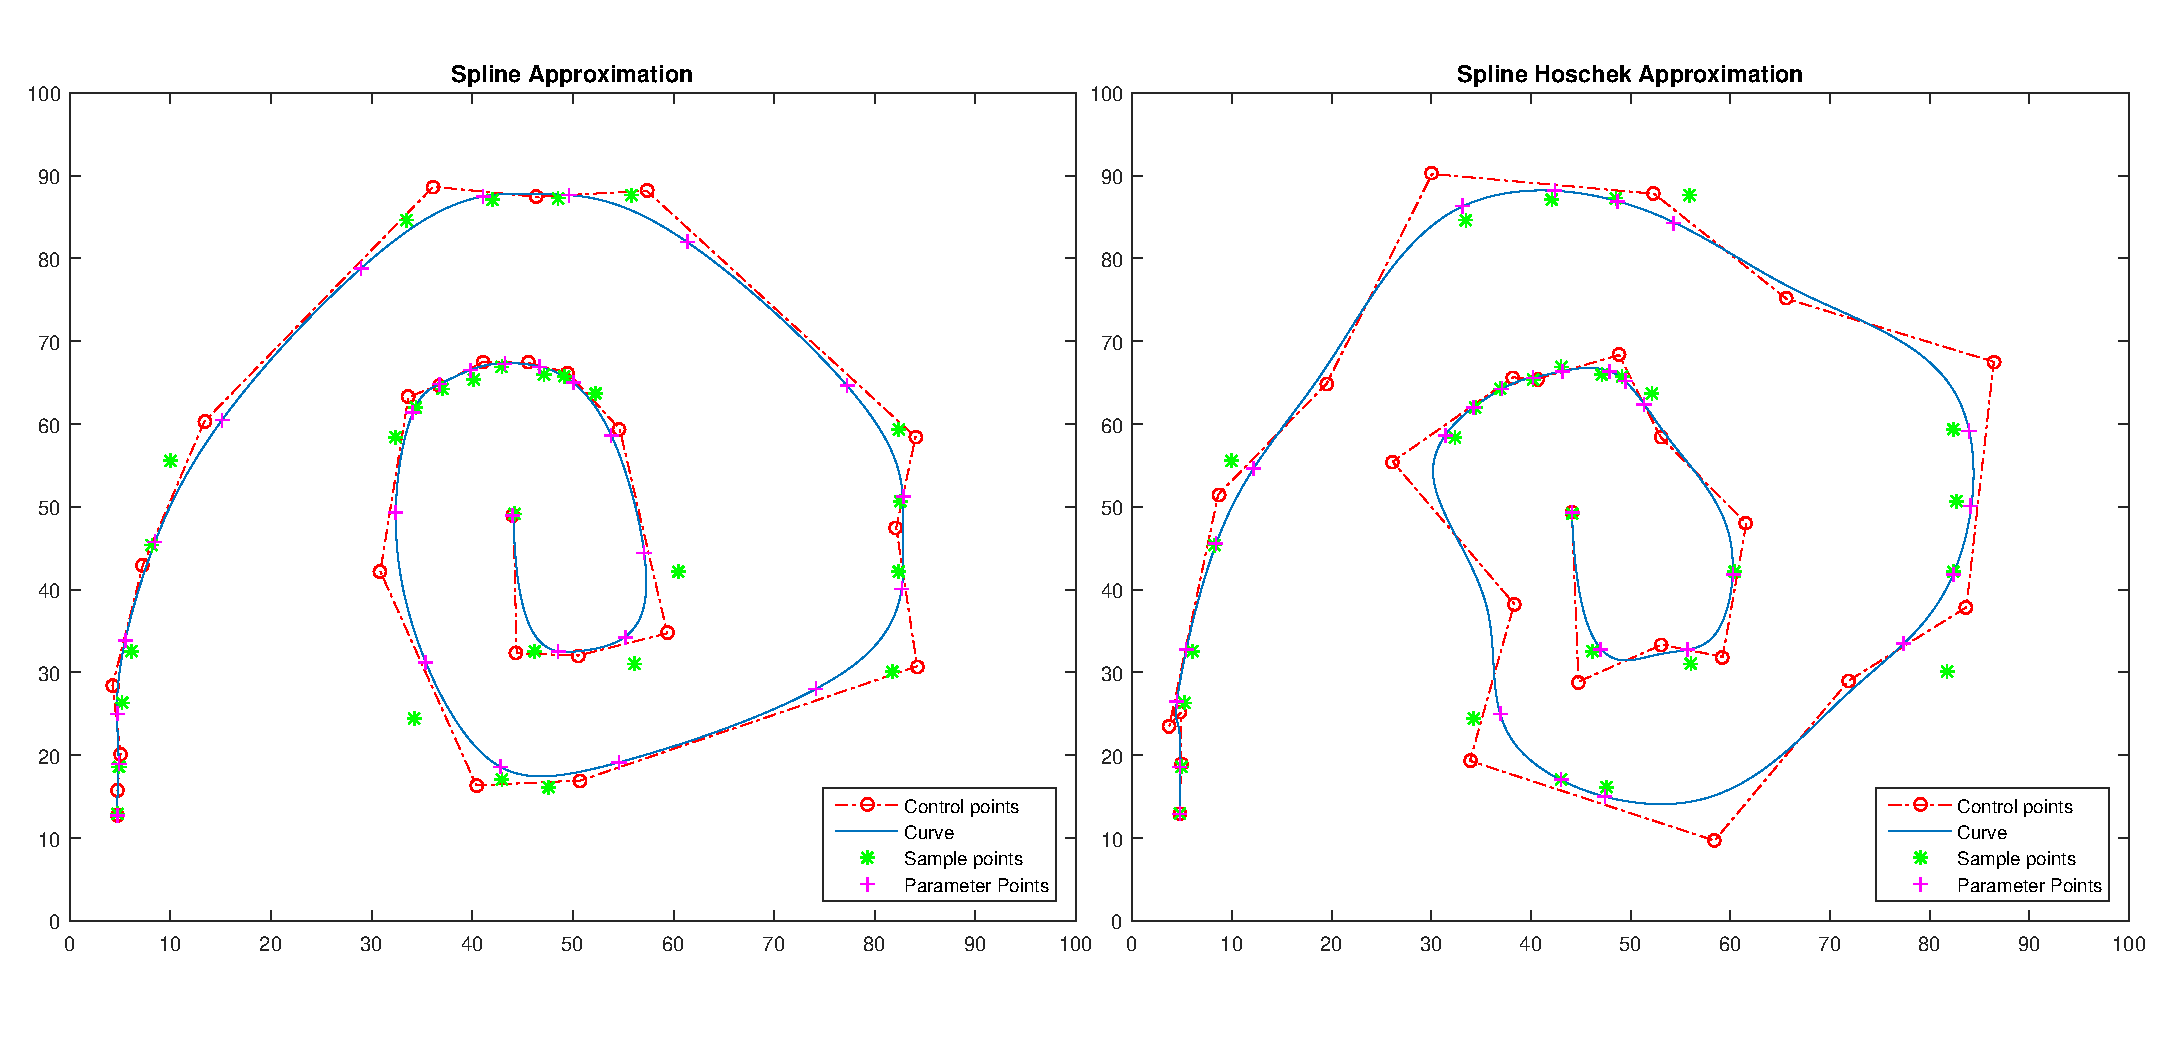
\includegraphics[width=\textwidth]{SplineApproximation.eps}
\caption{Two B-Splines of degree $3$ that approximate the data-points with $\lambda = 0.1$. The Hoschek algorithm stopped after $9$ iterations.}
\label{fig:splineApprox}
\end{figure}

\end{document}